%!TEX encoding = UTF-8 Unicode
%!TEX program = xelatex

\documentclass[bachelor]{ustcthesis}
% bachelor|master|doctor
\usepackage{ustcextra}
\graphicspath{{figures/}}
\bibliographystyle{ustcauthoryear}
% \bibliographystyle{ustcnumerical}


\newcommand{\docname}{xyz云盘系统}
\renewpagestyle{front}[\zihao{-5}]{
    \sethead{}{\docname 需求规格说明书}{}
    \setfoot{}{\thepage}{}
    \headrule
}
\renewpagestyle{main}[\zihao{-5}]{
    \sethead{}{\docname 需求规格说明书}{}
    \setfoot{}{\thepage}{}
    \headrule
}
\newcommand{\HRule}{\rule{\linewidth}{0.5mm}}

\begin{document}



\begin{titlepage}
\begin{center}
~\\[5cm]
\HRule \\[0.4cm]
{\huge \bfseries \docname\\需求规格说明书}\\[0.4cm]
\HRule \\[1.5cm]

\begin{tabular}{ccc}
  & 人员 & 日期 \\ 
拟制 & 宋小牛\ 陈泳洲\ 金泽文 & 2018-04-30 \\ 
评审人 & • & yyyy-mm-dd \\ 
批准 & • & yyyy-mm-dd \\ 
签发 & • & yyyy-mm-dd \\ 
\end{tabular} 

\end{center}
\end{titlepage}



\frontmatter
\begin{abstract}
本文档是xyz云盘系统需求规格分析文档,由
宋小牛、陈泳舟和金泽文共同创建,

本文档主要分析了该软件的总体概述、具体需求、总体设计约束、软件质量 特性、其他需求、依赖关系、需求分级和待确定问题等关于软件多个方面的需求。

\keywords{云盘\zhspace{} 分布式存储\zhspace{} 文件共享\zhspace{}  版本更新\zhspace{}
网络\zhspace{} 隐私\zhspace{} 安全\zhspace{}  p2p\zhspace{}  存储冗余\zhspace{} 内容审核\zhspace{} }
 
\begin{table}[htbp]
\centering
\caption{缩略词清单} \label{tab:abbr}
\begin{tabular}{|c|c|c|}
    \hline
    缩略语 & 英文全名 & 中文解释 \\
    \hline
    CentOS & Community Enterprise Operating Syste & 社区事业版操作系统\\
    \hline
    CSS & Cascading Style Sheets & 层叠样式表 \\
    \hline
    HTML & HyperText Markup Language & 超文本标记语言 \\
    \hline
    HTTP & HyperText Transfer Protocol & 超文本传输协议 \\
    \hline
    HTTPS & Hypertext Transfer Protocol Secure & 超文本传输安全协议 \\ 
    \hline
    IOPS & Input/Output Operations Per Second  & 每秒读写操作的次数\\
    \hline
    IP & Internet Protocol & 网际协议\\
    \hline
    MD5 & Message-Digest Algorithm 5 & 讯息摘要演算法 5\\
    \hline
    TCP & Transmission Control Protocol & 传输控制协议\\
    \hline
\end{tabular}
\end{table}

\end{abstract}

\tableofcontents
\listoffigures
\listoftables
% \listofalgorithms  % 算法索引,如不需要,可直接注释掉本行
% \input{chapters/notation}
\mainmatter
\chapter{简介}
\section{目的}
本需求规格说明书的阅读对象为xyz云盘系统的开发者和用户,其中,用户指的是掌握基本电脑操作的,有存储、上传、下载、共享文件的需求的人群。它详细地描述了xyz云盘系统的软件需求。

对于开发者,本文档主要用文字的方式,给开发者以清晰的开发思路,指明了xyz云盘系统开发时需要关注的要点重点,并且对该软件的具体功能需求、软件质量特性提出了详尽的方向。

对于用户,本文档主要提供xyz云盘系统可以提供的所有功能,以及相关接触特性,并且阐述了用户界面的使用方法,旨在给用户一个对于xyz云盘系统的整体认识与使用指导。

\section{范围}
本需求规格说明书主要包含了以下几个方面:

1.总体概述

2.具体需求

3.功能需求

4.总体设计约束

5.软件质量特性

6.其他需求

7.依赖关系

8.需求分级

9.待确定问题
\chapter{总体概述}

\section{软件概述}
\subsection{项目介绍}
云存储,是近几年在云计算的发展潮流之中诞生的,一项新兴的网络存储技术。云存储集成了网络技术和分布式文件系统等功能,是通过对不同的物理存储设备进行虚拟化映射,以形成逻辑层面统一的大存储空间的应用。

云盘系统,就是利用云存储技术,面向广大的有存储需求的客户,提供数据文件存储服务的第三方托管系统。

我们的xyz云盘系统,是基于分布式文件系统来设计和开发的云盘系统,是一个独立的项目。它的命名来自三位开发者名字的首字母(Xiaoniu,Yongzhou,Zewen),表明这将是由三位开发者开发的完全不同于其他云盘系统的新兴的云盘系统。

\subsection{产品环境介绍}

\begin{itemize}
	\item 本产品分为服务器端和客户端。服务器端作为后台运行程序,处理来自客户端的请求,进行数据存储,管理等;客户端作为客户发起请求。
	\item 服务器端需要用到MySQL,Ceph文件系统的接口;客户端和服务器端都需要HTTP/HTTPS协议支持。
	\item 服务器和客户端需要通信,双方都需要网络接口的支持。
\end{itemize}
\section{软件功能}

\subsection{普通用户}
\begin{itemize}
	\item 用户登录
	\item 编辑个人信息
	\item 上传文件资源
	\item 管理云端文件系统
	\item 发布资源链接
	\item 分享资源链接
	\item 下载资源
\end{itemize}

\subsection{游客}
\begin{itemize}
	\item 分享资源链接
	\item 下载资源
\end{itemize}

\section{用户特征}
\begin{itemize}
	\item 开发者与维护人员:具有相关的计算机专业知识,可以熟练地使用数据库,管理文件系统,并高效地解决软件异常。
	\item 普通用户:具备基本的浏览网页能力,认识中文并可以根据帮助理解基本的操作,可以操作图形界面。
	\item 游客:具备基本的浏览网页能力,明白如何下载链接,分享链接。
\end{itemize}

\section{假设和依赖关系}
\begin{itemize}
	\item 本产品客户端依赖于Windows/Linux/macOS等桌面操作系统或者移动平台操作系统,及各平台下的浏览器。
	\item 本产品服务器端依赖于MySQL数据库,Debian Linux操作系统,Java语言及相关库。
	\item 本产品通信依赖于HTTP/HTTPS协议。
\end{itemize}

\chapter{具体需求}
\section{功能需求}

本章节描述xyz云盘系统所必须执行的基本动作,以及其输入、输出,以及中间处理的过程。
\subsection{R.XYZ.CLOUDSTORAGE.USER.LOGIN.001 用户:显示初始登陆界面 }

\subsubsection{介绍}
打开客户端之后,用户需要登陆,才可以访问自己的存储数据。登陆需要友好的登录界面。

\subsubsection{输入}
用户打开客户端。

\subsubsection{处理}
生成登录窗口,包括用户名密码等窗口,其中,密码需要密码显示的保护处理。
\subsubsection{输出}
显示友好的登录窗口。

\subsection{R.XYZ.CLOUDSTORAGE.USER.LOGIN.002 用户:密码验证 }

\subsubsection{介绍}
在看到登陆界面之后,用户需要输入用户名密码,并通过”登陆“键提交密码,以进行验证并登陆。

\subsubsection{输入}
用户输入用户名和密码,按”登陆“键,或者”Enter“键。

\subsubsection{处理}
客户端将用户名密码,结合时间戳进行密码学处理之后打包,发送给服务器端。
服务器端通过密码学手段验证密码。如果密码正确,返回带有时间戳的cookie给客户端。如果密码错误,则返回错误信息给客户端。错误次数不能超过4次。超过则禁止ip尝试同一用户。如果发生通信异常,则保存异常信息到异常日志中,同时客户端重传,直到超时。

\subsubsection{输出}
如果密码正确,显示用户的根文件夹;如果密码错误,显示”密码错误“,以及错误次数,进行警告。如果通信异常,则显示通信异常信息。

\subsection{R.XYZ.CLOUDSTORAGE.USER.LOGOUT.001 用户:退出 }

\subsubsection{介绍}
用户能够退出客户端,结束本次使用。

\subsubsection{输入}
用户按下“退出”按钮,或者直接关闭客户端。

\subsubsection{处理}
用户“按下退出”按钮后,客户端发包给服务器端,提示结束本次使用。服务器端将该用户设置为“离线”状态。
用户通过其他方式直接关闭客户端时(包括强制关闭,关机等),服务器端定期检查客户端是否在线,如果超时无回应,则自动设置为“离线”状态。

\subsubsection{输出}
客户端被关闭。

\subsection{R.XYZ.CLOUDSTORAGE.FILE.BASIC.001 文件:打开文件夹}

\subsubsection{介绍}
用户可以打开文件夹,查看所包含的文件及子文件夹。

\subsubsection{输入}
用户双击文件夹,或者选中文件夹之后点击打开选项。

\subsubsection{处理}
客户端将打开文件夹的指令打包,发送到服务器,服务器传回文件夹内容。客户端接收之后,切换路径到所选中的文件夹,并展示其所包含的文件及文件夹。

异常:如果通信失败,则客户端重传,直到超时。

\subsubsection{输出}
若无异常发生,用户可以看到文件夹中的文件以及子文件夹。

若有异常发生,则将异常信息保存到日志中,并显示友好界面提示异常。

\subsection{R.XYZ.CLOUDSTORAGE.FILE.BASIC.002 文件:查看文件属性}

\subsubsection{介绍} 
用户可以查看文件属性,包括文件大小、创建时间、修改时间、上次下载时间、上次访问时间、md5值等。

\subsubsection{输入} 
用户选中文件,再点击属性选项。

\subsubsection{处理}
客户端将该请求发送到服务器端,服务器查询属性,并传回客户端。客户端显示属性值。
异常:如果通信失败,则客户端重传,直到超时。
若有异常发生,则将异常信息保存到日志中,并显示友好界面提示异常。

\subsubsection{输出}
客户端接收到之后弹窗显示各项属性值。


\subsection{R.XYZ.CLOUDSTORAGE.FILE.BASIC.003 文件:排序显示}

\subsubsection{介绍} 
用户可以按照文件名以及属性值选择排序显示的方式。

\subsubsection{输入} 
用户点击“排序”选项,并选中所要排序的依据。

\subsubsection{处理}
客户端按照用户的选择,调用排序函数,排好序之后进行显示。

\subsubsection{输出}
客户端按照排序结果显示文件和文件名。



\subsection{R.XYZ.CLOUDSTORAGE.FILE.BASIC.004 文件:重命名}

\subsubsection{介绍} 
用户可以对文件以及文件夹进行重命名操作。

\subsubsection{输入} 
用户选中文件或文件名,右键,选中“重命名”选项。

\subsubsection{处理}
客户端将重命名的原名字和新名字打包发给服务器端,服务器检查该重命名是否合法不冲突,是则返回“成功”的信息,否则,返回“失败”的信息。

异常:如果通信失败,则客户端重传,直到超时。
若有异常发生,则将异常信息保存到日志中,并显示友好界面提示异常。

\subsubsection{输出}
如果成功,则刷新当前目录,显示最新的名字。如果失败,则提示失败。


\subsection{R.XYZ.CLOUDSTORAGE.FILE.BASIC.005 文件:复制、粘贴、剪切}

\subsubsection{介绍} 
用户可以对部分文件以及文件夹进行复制、粘贴、剪切等操作。

\subsubsection{输入} 
复制:用户选中需要操作的文件和文件夹,右键,选中“复制”选项。

剪切:用户选中需要操作的文件和文件夹,右键,选中“剪切”选项。

粘贴:用户在所要粘贴的文件夹中,右键,选中“粘贴”选项。需要注意的是,必须有之前“复制”或“剪切”的操作记录,“粘贴”选项才可选。

\subsubsection{处理}
复制:客户端将用户选中要复制的项的完全名字(包括路径)存储到cache中。

剪切:客户端将用户选中要剪切的项的完全名字(包括路径)存储到cache中。

粘贴:客户端将执行粘贴的文件夹的路径,以及之前复制或者剪切的类型一起打包,发给服务器端。服务器接收之后检查命名是否冲突。如果冲突就返回“命名冲突”信息;如果不冲突,如果是复制,则复制到目标文件夹,如果是剪切,则先复制,再删除。最后返回“成功”给客户端。

\subsubsection{输出}
如果粘贴成功,则刷新当前文件夹,显示最新结果。
如果粘贴失败,则弹窗提示粘贴失败。

\subsection{R.XYZ.CLOUDSTORAGE.FILE.HIGH.001 文件:回收站}

\subsubsection{介绍} 
用户可以将文件以及文件夹移入回收站,回收站在7天后自动删除,用户也可以在回收站住主动删除。用户也可以讲文件以及文件夹从回收站中移出。

\subsubsection{输入} 
移入回收站:用户选中文件或文件夹,右键,选中“移入回收站”选项。

移出回收站:用户在回收站中选中文件或文件夹,右键,选中“移出回收站”选项。

彻底删除:用户在回收站中选中文件或文件夹,右键,选中“彻底删除”。

\subsubsection{处理} 
移入回收站:客户端将该文件或文件夹名字打包发送到服务器端。服务器将该文件或文件夹移入“回收站”中并返回“成功”。客户端收到信息后,刷新当前文件夹。如果超时,则弹窗提示。

移出回收站:客户端将该文件或文件夹名字打包发送到服务器端。服务器端检查该文件或文件夹复原之后是否有命名冲突等。如果无冲突则移出“回收站”中并返回“成功”,否则返回“失败”。客户端收到信息后,如果成功,则刷新回收站;如果失败,则弹窗提示。

彻底删除:客户端将该文件或文件夹名字打包发送到服务器端。服务器从回收站中删除。返回“成功”。客户端收到信息后,如果成功,则刷新回收站;如果失败,则弹窗提示。

异常:如果通信失败,则客户端重传,直到超时。
若有异常发生,则将异常信息保存到日志中,并显示友好界面提示异常。

\subsubsection{输出} 
移入回收站:如果成功,则刷新当前文件夹,否则弹窗提醒。

移出回收站:如果成功,则刷新回收站,否则弹窗提醒。

彻底删除:如果成功,则刷新当前文件夹,否则弹窗提醒。

\subsection{R.XYZ.CLOUDSTORAGE.FILE.HIGH.002 文件:收藏夹}

\subsubsection{介绍} 
用户可以将文件以及文件夹加入收藏夹,以便快速访问。

\subsubsection{输入} 
加入收藏夹:用户选中文件或文件名,右键,选中“加入收藏夹”选项。
移出收藏家:用户在收藏夹中选中文件或文件名,右键,选中“移出收藏夹”选项。

\subsubsection{处理}
加入收藏夹:客户端将用户选中的文件名打包发给服务器端,服务器将该文件或文件夹加入所维护的收藏夹数据结构中。返回成功。
移出收藏夹:客户端将用户选中的文件名打包发给服务器端,服务器将该文件或文件夹从所维护的收藏夹数据结构中删除。返回成功。
异常:如果通信失败,则客户端重传,直到超时。
若有异常发生,则将异常信息保存到日志中,并显示友好界面提示异常。

\subsubsection{输出}
如果成功,并且是当前目录是收藏夹,则刷新当前目录,显示最新的名字。如果失败,则提示失败。

















逐条列出与本特性相关的功能需求。包括项目如何响应预期的错误输入,非法条件和无效输入。需求应该简明,完整,不含糊,可验证,必要的。 当需要的信息不确定的时候使用“待定”。
\subsubsection{输入}
This section consists of:
A. Detailed description of all input data of the function, including:
Source of input
Quantify
Measurement units
Timing requirements
Valid input range that contains the precision and tolerance
B. Reference of interface specification or interface control document that are provided in proper place.

本子段落应包含下列内容:

A. 对该功能所有输入数据的详细描述,包括:

		输入来源
		数量
		度量单位
		时间要求
		包含精度和容忍度的有效输入范围
		
B. 在适当的地方提供的对接口规格或接口控制文档的参考。
\subsubsection{处理}
Describes all the operations on the input data, and the process to get the output data, including the following specifications:
A. Verification of input data
B. Exact order of the operations, including the time sequene of each event.
C. Response to exception, such as:
		 Overflow
		Communication failure
		Error process
D. Any method used to transfer the input data to the output data. (such as equation,mathematic algorithm and logical operation)
For example.
		The formula to calculate the income tax in a pay roll.
		the weather model used for weather forecast
E. Verification of output data.
本子段落应描述对输入数据所执行的所有操作和如何获得输出的过程。这包括下列规格:

A. 输入数据的有效性检测。

B. 操作的确切次序,包括各事件的时序。

C. 对异常情况的回应,例如:
		溢出
		通信失败
		错误处理
D. 用于把系统输入转换到相应输出的任何方法(诸如方程式,数学算法,逻辑操作)。例如,这可能描述下列方面:
		对工资单里代扣所得税的计算公式。
		用于气象预报的气象模型。
		
E.	对输出数据的有效性检测。
\subsubsection{输出}
This section should include:
A. The detailed description of output data of the function, including:
		Target to output to (Such as a printer or a file)
		Quantity
		Measurement units
		Time sequence
		Valid output range including the precision and tolerance
		Process of the invalid value.
		Error message.
B. Reference of interface specification or interface control document that are provided in proper place.
For the systems with their requirements focused on the input/output actions, all the important input/output actions and the time sequences of the input/output pairs should be described in the SRS. In a system that inputs and actions are memorized as the basis for the reactions to be taken, the timing sequence for the input/output pairs must be available here. This kind of functional action is similar to a status machine.  
本子段落应包含:

A. 对该功能所有输出数据的详细描述,这个描述包括:
		输出的到何处(如打印机,文件)
		数量
		度量单位
		时序
		包含精确度和容忍度的有效输出范围
		对非法值的处理
		错误消息
		
B. 在适当的地方提供对接口规格或接口控制文档的参考。

此外,对那些需求集中在输入/输出行为的系统,SRS应描述所有重要的输入/输出行为及输入输出对的次序。对一个需要记忆其行为以根据输入和过去的行为进行反应的系统,输入输出对的次序是要求的;这种功能行为就类似于有限状态机。

\section{性能需求}

\subsection{服务器性能需求}
 
1. 云盘拥有公网ip,供全网用户访问,并发量应做到:允许1000用户同时访问网盘,并保证浏览指定文件夹的文件能在1s内完成

2. 本云盘为方便用户在不同终端访问文件与进行文件备份,故对磁盘存储空间要求较高:单个用户至少1TB,总空间在500TB左右。单用户文件数量在数百个左右,总数量在5000左右。

3. 至少需要1Gbps的有线互联网接入,以保证每个用户的下载速度

4. 为防止服务器宕机使得数据丢失,需要提供冗余机制

\subsection{客户端性能需求}

1. 用户使用普通浏览器访问网盘,不需要太高性能,普通智能手机与商务电脑即可支持

2. 用户端至少需要200KB/s的下载/上传网速来保证文件的正常下载、上传

\section{外部接口需求}
\subsection{用户接口}

用户使用浏览器访问给定的域名来访问云盘,在不同size的屏幕上自适应,支持Chrome,Edge,Firefox等主流浏览器。

对计算机基本使用较为熟悉的用户可以在不需要他人教学的情况下,10分钟能自主学会使用本软件

使用方式:
1. 上传、下载、删除重命名等功能按钮与右键菜单
2. 拖拽、复选框进行复选

在这里插入软件界面示意图

\subsection{软件接口}
<The interface with other system/modules/projects should be explained in detail. >

详细描述与其他系统 /模块 /项目之间的接口

Describes how to use the other (required) software products. (such as data management system, operation system, or algorithm tools package), and the interfaces to other application systems (such as interfaces between the protocol process system and the database management system )
For each required software product, following information should be provided:
A. Name
B. Mnemonic symbol
C. Version number
D. Source
For each interface, this section should:
A. Discuss the objective of the required software.
B. Define the interfaces by content and format of message/function. If the interfaces have been clearly described in other documents, it is not necessary to describe in detail here. But the reference of those documents should be given.

在此应描述如何使用其它(必需的)软件产品(例如,数据管理系统,操作系统,或算法工具包),以及与其它应用系统的接口(例如,协议处理系统和数据库管理系统之间的接口)。

对每个必需的软件产品,应提供下列信息:
A.	名字
B.	助记符
C.	版本号
D.	来源

对每个接口,本部分应:

A .	讨论与本软件产品相关的接口软件的目的。

B.	按消息/函数内容和格式定义接口。如果接口已在其它文档中很清楚地描述,就没有必要在这儿进行详细描述,但需说明应参考的文档。

\subsection{硬件接口}
<The interface with other hardware components should be explained in detail. >

详细描述与硬件的接口

Describes the logical features of the interface between the software and hardware components, including the equipment supported and how the equipment and protocol is supported. 

Defines the interfaces according to the content and format of the software/hardware protocol. If the interfaces have been clearly described in other documents, it is not necessary to describe in detail here. But the reference of those documents should be given.

在此描述软件产品和系统硬件组件之间接口的逻辑特征,也包括支持哪些设备、怎样支持这些设备和协议等。
 
按软/硬件协议内容和格式定义接口。如果接口已在其它文档中很清楚地描述,就没有必要在这儿进行详细描述,但需说明应参考的文档。

\subsection{通讯接口}
<This should specify the various interfaces to communications such as local network protocols, etc.>

详细描述通讯接口,如本地网络协议等。

Defines the interfaces according to the content and format of the message/function. If the interfaces have been clearly described in other documents, it is not necessary to describe in detail here. But the reference of those documents should be given.

按消息/函数内容和格式定义接口。如果接口已在其它文档中很清楚地描述,就没有必要在这儿进行详细描述,但需说明应参考的文档。

\chapter{总体设计约束}
 
\section{标准符合性}
\begin{itemize}
  \item 后端开发符合Oracle Java code conventions 编码规范
  \item 前端开发符合 W3C-HTML5 编码规范
  \item UI设计符合MaterialDesign规范
\end{itemize}

\section{硬件约束}
\begin{itemize}
  \item 服务器端:Debian 操作系统,E5 处理器,64GB 内存,1Gbps 及以上的网络接入 
  \item 客户端:Windows/Linux/macOS 等桌面操作系统,1GB 及以上内存,需要安装浏览器;或者iOS/Android等移动平台操作系统,1GB 及以上内存,需要安装浏览器
\end{itemize}

\section{技术限制}
\begin{itemize}
  \item 后端开发:Java SE 10/Ceph
  \item 前端开发:HTML5/JQuery/CSS
  \item UI设计风格:MaterialDesign风格
  \item 通讯协议:TCP/IP
  \item 网络协议:HTTP/HTTPS
  \item 并行操作:支持
\end{itemize}
\chapter{软件质量特性}

\section{适应性}

本云盘可以在移动平台、桌面平台访问,只需要一个通用的浏览器即可,覆盖了基本所有的使用场景

\section{可用性}

本云盘可提供99.9\%的可用性,即连续运行一年时间里期望中断时间是8.76小时:这依赖于底层文件系统的高可用性与操作系统的稳定性以及网络链接的稳定性

\section{安全性}

本云盘系统使用加密链接,防止技术层面上的信息泄露。同时有着完善的权限管理,防止用户绕过权限对不可见、不可修改的文件进行操作。

\section{正确性}

云盘建立在TCP链接上,已有基础的正确性保证的同时还会对数据传输加上CRC校检码,保证数据传输的正确性

\section{灵活性}

本云盘能适应多种不同的操作、应用场景,满足不同用户的操作习惯:
在线解压、压缩,多种方式复选,鼠标拖拽复选、移动

同时本云盘还提供上传、下载的断点续传功能

\section{交互工作能力}

本云盘的交互方式繁多但易用:

1. 复选框

2. 右键操作与功能按钮操作

3. 多种排列方式显示

4. 缩放

5. 多个标签页

允许用户灵活的组合各个功能来使用本云盘,实现复杂操作

\section{可维护性}

本云盘系统尽最大努力实现机制与策略分离,各个模块之间低耦合,方便后期调整策略、维护

\section{可移植性}

本云盘系统的客户端为网页,从而可以在任意平台上使用。服务器端则能适配大多数Linux平台

{
\color{red}
\section{可靠性}

本云盘系统对绝大多数应用场景中会出现的异常情况做了包容处理,以及多个用户对公共文件的同时处理的包容,通过跨磁盘的存储冗余机制,绝对地降低了系统宕机的可能性,使可靠性得到保证
}

\section{可重用性}

本云盘的各个模块对其他模块的依赖性都被尽量降低,使得其可以方便的重用到其他项目中

\section{鲁棒性}

本云盘除了对请求进行校验,还将对多种网络攻击手段进行预防,避免异常行为的发生影响系统运行和用户使用

\section{可测试性}

本云盘系统的各个模块都经过了完善的测试,保证能经受用户的各种操作而稳定运行

\chapter{其他需求}

使用适当的章节,详细说明任何其他客户需求,包括数据库,编码需求,错误处理,测试需求等。下面仅列出了少量样例,你可以删除和增加项目。
\section{数据库}

详细说明项目相关的数据库方面的需求。
\section{操作}
<This could specify the normal and special operations required by the user. >

详细说明用户通常的和特殊的操作需求。
\section{本地化}
<Any requirement on multi language operation could be described here. >

描述支持多语种的需求。

\chapter{依赖关系}

\begin{table}[htbp]
\centering
\caption{功能需求的依赖关系表} \label{tab:simpletable}
\begin{tabular}{|c|c|c|}
    \hline
    依赖部分 & 被依赖部分 & 解释  \\
    \hline
    R..USER.LOGIN.002 & R..USER.LOGIN.001 & 显示初始登录界面之后才可以验证密码 \\
    \hline
    R..USER.LOGIN.003 & R..USER.LOGIN.001 & 显示初始登录界面之后才可以注册 \\
    \hline
    R..USER.LOGIN.004 & R..USER.LOGIN.001 & 显示初始登录界面之后才可以重置密码 \\
    \hline
    R..USER.LOGIN.005 & R..USER.LOGIN.002 & 用户登录之后才可以退出 \\
    \hline
    R..FILE & R..USER.LOGIN.002 & 所有的文件操作(除了游客\\ &  &操作之外)都需要用户登录 \\ 
    \hline
    R..SHAREFOLDER & R..USER.LOGIN.002 & 所有的共享文件夹操作(除了\\ &  &游客操作之外)都需要用户登录\\
    \hline
    R..FILE.BASIC.002 & R..FILE.BASIC.001 & 用户下载之前该文件/文件夹要被上传 \\
    \hline
    R..FILE.BASIC.002 & R..FILE.BASIC.004 & 或者用户下载之前该文件/文件夹要被分享 \\
    \hline
    R..FILE & R..FILE.HIGH.003 & 对于加密的文件或文件夹,\\ &  & 用户操作之前还要输入密码进行确认\\
    \hline
    R..FILE.HIGH.011 & R..FILE.HIGH.010 & 审核系统需要部分依赖举报功能 \\
    \hline
    
\end{tabular}
\note{表中的R..XXX等均指R.XYZ.CLOUDSTORAGE.XXX}
\end{table} 


\begin{table}[htbp]
\centering
\caption{性能需求的依赖关系表} \label{tab:simpletable}
\begin{tabular}{|c|c|c|}
    \hline
    依赖部分 & 被依赖部分 & 解释  \\
    \hline
    网络带宽、延迟 & 网络硬件环境, & 高带宽、低延迟,要求极高的网络环境 \\
    & 服务器网络结构 &  \\
    \hline
    用户存储空间 & 磁盘硬件大小 & 足够的用户存储空间需要足够的磁盘容量、数量 \\
    \hline
    存储冗余 & Ceph文件系统 & 可靠高效的存储冗余需要利用Ceph文件系统 \\
    \hline
    客户端的运行 & 用户终端硬件基础 & 客户端需要至少200kB/s的带宽,\\ & & 以及1GB以上的内存 \\
    \hline
    
\end{tabular}
\end{table} 




\begin{table}[htbp]
\centering
\caption{外部接口的依赖关系表} \label{tab:simpletable}
\begin{tabular}{|c|c|c|}
    \hline
    依赖部分 & 被依赖部分 & 解释  \\
    \hline
    客户端的运行 & 用户终端软件基础 & 客户端需要运行在主流操作系统上:\\ & & 如:Linux、MacOS、Windows \\ & & 客户端需要运行在主流浏览器中: \\ & & 如:Chrome、Edge、Firefox \\
    \hline
    数据管理系统 & Mysql & 优质的开源DBMS \\
    \hline
    服务器操作系统 & CentOS & 以稳定出名的开源操作系统\\
    \hline
    分布式文件系统 & Ceph & 以稳定高效高可用出名的分布式文件系统\\
    \hline
    HTTP服务器 & Tomcat & 以便捷高效出名的Apache项目 \\
    \hline
    后端框架语言 & Java & 使用量最多的编程语言\\
    \hline
    服务器架构 & x64集群或云主机 & 需要庞大数量的服务器\\
    \hline
    通讯接口 & HTTP/HTTPS,TCP/IP协议 & 网络应用必备的协议 \\
    \hline
    
\end{tabular}
\end{table} 



    
\chapter{需求分级}
\begin{table}[htbp]
    \color{red}
\centering
\caption{需求分级表1} \label{tab:abbr}
\begin{tabular}{|c|c|c|}
    \hline
    需求ID & 需求名称 & 需求分级 \\
    \hline
    R..USER.LOGIN.001 & 用户:初始界面 & 必须 \\
    \hline
    R..USER.LOGIN.002 & 用户:密码验证 & 必须 \\
    \hline 
    R..USER.LOGIN.003 & 用户:注册 & 必须 \\
    \hline
    R..USER.LOGIN.004 & 用户:忘记密码 & 重要 \\
    \hline
    R..USER.LOGIN.005 & 用户:退出 & 必须 \\
    \hline
    R..USER.MEMBERSHIP.001 & 用户:开通会员 & 必须 \\
    \hline
    R..USER.MEMBERSHIP.002 & 用户:开通会员 & 重要 \\
    \hline
    R..USER.MEMBERSHIP.003 & 用户:优惠券活动 & 必须 \\
    \hline
    R..USER.SOCIAL.001 & 用户:搜索用户 & 必须 \\
    \hline
    R..USER.SOCIAL.002 & 用户:添加好友 & 必须 \\
    \hline
    R..USER.SOCIAL.003 & 用户:个人隐私设置 & 必须 \\
    \hline
    R..FILE.BASIC.001 & 文件:上传 & 必须 \\
    \hline
    R..FILE.BASIC.002 & 文件:下载 & 必须 \\
    \hline 
    R..FILE.BASIC.003 & 文件:新建文件夹 & 重要 \\
    \hline
    R..FILE.BASIC.004 & 文件:打开文件夹 & 必须 \\
    \hline
    R..FILE.BASIC.005 & 文件:返回上级文件夹 & 必须 \\
    \hline
    R..FILE.BASIC.006 & 文件:查看文件属性 & 重要 \\
    \hline
    R..FILE.BASIC.007 & 文件:排序显示 & 重要 \\
    \hline
    R..FILE.BASIC.008 & 文件:重命名 & 重要 \\
    \hline
    R..FILE.BASIC.009 & 文件:复制、剪切、粘贴 & 重要 \\
    \hline
    R..FILE.BASIC.010 & 文件:创建,关闭标签页 & 最好有的 \\
    \hline
    R..FILE.BASIC.011 & 文件:基本分类 & 必须 \\
    \hline
    R..FILE.BASIC.012 & 文件:会员加速 & 必须 \\
    \hline
    R..FILE.HIGH.001 & 文件:回收站 & 必须 \\
    \hline
    R..FILE.HIGH.002 & 文件:收藏夹 & 重要 \\
    \hline
    R..FILE.HIGH.003 & 文件:加密 & 重要 \\
    \hline
    R..FILE.HIGH.004 & 文件:分享 & 必须 \\
    \hline
    R..FILE.HIGH.005 & 文件:分类 & 最好有的 \\
    \hline 
\end{tabular}
\note{表中的R..XXX等均指R.XYZ.CLOUDSTORAGE.XXX}
\end{table}
\begin{table}[htbp]
\centering
\caption{需求分级表2} \label{tab:abbr}
\begin{tabular}{|c|c|c|}
    \hline
    需求ID & 需求名称 & 需求分级 \\
    \hline
    R..FILE.HIGH.006 & 文件:搜索 & 重要 \\
    \hline
    R..FILE.HIGH.007 & 文件:预览 & 最好有的 \\
    \hline
    R..FILE.HIGH.008 & 文件:在线解压 & 最好有的 \\
    \hline
    R..FILE.HIGH.009 & 文件:在线压缩 & 最好有的 \\
    \hline
    R..FILE.HIGH.010 & 文件:举报 & 最好有的 \\
    \hline
    R..FILE.HIGH.011 & 文件:审核 & 最好有的 \\
    \hline
    R..TAB.001 & 标签页:创建 & 最好有的 \\
    \hline
    R..TAB.002 & 标签页:关闭 & 最好有的 \\
    \hline
    R..SHAREFOLDER.001 & 共享文件夹:创建 & 重要 \\
    \hline
    R..SHAREFOLDER.002 & 共享文件夹:打开 & 重要 \\
    \hline
    R..SHAREFOLDER.003 & 共享文件夹:权限匹配 & 最好有的 \\
    \hline
    R..SHAREFOLDER.004 & 共享文件夹:权限管理 & 最好有的 \\
    \hline
    R..VERSION.001 & 版本管理:版本更新 & 重要 \\
    \hline
\end{tabular}
\note{表中的R..XXX等均指R.XYZ.CLOUDSTORAGE.XXX}
\end{table}

\chapter{待确定问题}
\begin{table}[htbp]
\centering
\caption{待确定问题表} \label{tab:tbd_problems}
\begin{tabular}{|c|p{3cm}|p{1cm}|c|p{3cm}|p{1cm}|p{1cm}|}
    \hline
    需求ID & 问题描述 & 影响(H/M/L) & 风险 & 责任人 & 解决日期 & 状态(Open/ Close) \\
    \hline
    R..FILE.BASIC.001 & 文件上传中途失败如何处理 & M & 中 & 宋小牛、金泽文、陈泳舟 & - & Open\\
    \hline
    R..FILE.BASIC.002 & 如何分段传输过大的文件 & H & 高 & 宋小牛、金泽文、陈泳舟 & - & Open\\
    \hline
    R..FILE.BASIC.007 & 如何选择具体的排序顺序 & L & 低 & 宋小牛、金泽文、陈泳舟 & - & Open\\
    \hline
    R..FILE.HIGH.001 & 是否定期清理回收站 & M & 中 & 宋小牛、金泽文、陈泳舟 & - & Open\\
    \hline
    R..FILE.HIGH.003 & 如何选择合适的加密算法 & M & 中 & 宋小牛、金泽文、陈泳舟 & - & Open\\ 
    \hline
    R..FILE.HIGH.007 & 可以预览的文件类型 & L & 低 & 宋小牛、金泽文、陈泳舟 & - & Open\\
    \hline
    R..FILE.HIGH.011 & 如何高效识别非法内容 & H & 高 & 宋小牛、金泽文、陈泳舟 & - & Open\\
    \hline
    R..TAB.001 & 新标签页如何排版 & L & 低 & 宋小牛、金泽文、陈泳舟 & - & Open\\
    \hline
    R..SHAREFOLDER.003 & 读写子目录是否需要父目录权限 & L & 低 & 宋小牛、金泽文、陈泳舟 & - & Open\\
    \hline
    
\end{tabular}
\note{表中的R..XXX等均指R.XYZ.CLOUDSTORAGE.XXX}
\end{table}
% \chapter{Latex使用例子}

\section{图}
\subsection{示例}
\begin{figure}[ht]
\centering

\includegraphics[width=10cm]{ustc_logo_fig}
\caption{测试图片} \label{fig:figure1}
\end{figure}

\subsection{带图注的图}
\begin{figure}[ht]
\centering

\includegraphics[width=10cm]{ustc_logo_fig}
\caption{带图注的图片}\label{fig:noted-figure}
\note{the solid lines represent the time histogram of the spontaneous activities of an old monkey cell(gray) and a young monkey cell (black). The bin-width is 1}
\end{figure}

\section{表格}

\subsection{A Simple Table}
\begin{table}[htbp]
\centering
\caption{这里是表的标题} \label{tab:simpletable}
\begin{tabular}{|c|c|}
    \hline
    a & b \\
    \hline
    c & d \\
    \hline
\end{tabular}
\note{这里是表的注释}
\end{table}

\subsection{长表格}
\begin{longtable}{ccc}
% 首页表头
\caption[长表格演示]{长表格演示} \label{tab:longtable} \\
\toprule[1.5pt]
名称  & 说明 & 备注\\
\midrule[1pt]
\endfirsthead
% 续页表头
\caption[]{长表格演示(续)} \\
\toprule[1.5pt]
名称  & 说明 & 备注 \\
\midrule[1pt]
\endhead
% 首页表尾
\hline
\multicolumn{3}{r}{\small 续下页}
\endfoot
% 续页表尾
\bottomrule[1.5pt]
\endlastfoot

AAAAAAAAAAAA   &   BBBBBBBBBBB   &   CCCCCCCCCCCCCC   \\
AAAAAAAAAAAA   &   BBBBBBBBBBB   &   CCCCCCCCCCCCCC   \\
AAAAAAAAAAAA   &   BBBBBBBBBBB   &   CCCCCCCCCCCCCC   \\
AAAAAAAAAAAA   &   BBBBBBBBBBB   &   CCCCCCCCCCCCCC   \\
AAAAAAAAAAAA   &   BBBBBBBBBBB   &   CCCCCCCCCCCCCC   \\
AAAAAAAAAAAA   &   BBBBBBBBBBB   &   CCCCCCCCCCCCCC   \\
AAAAAAAAAAAA   &   BBBBBBBBBBB   &   CCCCCCCCCCCCCC   \\
AAAAAAAAAAAA   &   BBBBBBBBBBB   &   CCCCCCCCCCCCCC   \\
AAAAAAAAAAAA   &   BBBBBBBBBBB   &   CCCCCCCCCCCCCC   \\
AAAAAAAAAAAA   &   BBBBBBBBBBB   &   CCCCCCCCCCCCCC   \\
AAAAAAAAAAAA   &   BBBBBBBBBBB   &   CCCCCCCCCCCCCC   \\
AAAAAAAAAAAA   &   BBBBBBBBBBB   &   CCCCCCCCCCCCCC   \\
AAAAAAAAAAAA   &   BBBBBBBBBBB   &   CCCCCCCCCCCCCC   \\
AAAAAAAAAAAA   &   BBBBBBBBBBB   &   CCCCCCCCCCCCCC   \\
AAAAAAAAAAAA   &   BBBBBBBBBBB   &   CCCCCCCCCCCCCC   \\
AAAAAAAAAAAA   &   BBBBBBBBBBB   &   CCCCCCCCCCCCCC   \\
AAAAAAAAAAAA   &   BBBBBBBBBBB   &   CCCCCCCCCCCCCC   \\
AAAAAAAAAAAA   &   BBBBBBBBBBB   &   CCCCCCCCCCCCCC   \\
AAAAAAAAAAAA   &   BBBBBBBBBBB   &   CCCCCCCCCCCCCC   \\
AAAAAAAAAAAA   &   BBBBBBBBBBB   &   CCCCCCCCCCCCCC   \\
AAAAAAAAAAAA   &   BBBBBBBBBBB   &   CCCCCCCCCCCCCC   \\
AAAAAAAAAAAA   &   BBBBBBBBBBB   &   CCCCCCCCCCCCCC   \\
AAAAAAAAAAAA   &   BBBBBBBBBBB   &   CCCCCCCCCCCCCC   \\
AAAAAAAAAAAA   &   BBBBBBBBBBB   &   CCCCCCCCCCCCCC   \\
AAAAAAAAAAAA   &   BBBBBBBBBBB   &   CCCCCCCCCCCCCC   \\
AAAAAAAAAAAA   &   BBBBBBBBBBB   &   CCCCCCCCCCCCCC   \\
AAAAAAAAAAAA   &   BBBBBBBBBBB   &   CCCCCCCCCCCCCC   \\
AAAAAAAAAAAA   &   BBBBBBBBBBB   &   CCCCCCCCCCCCCC   \\
AAAAAAAAAAAA   &   BBBBBBBBBBB   &   CCCCCCCCCCCCCC   \\
AAAAAAAAAAAA   &   BBBBBBBBBBB   &   CCCCCCCCCCCCCC   \\
AAAAAAAAAAAA   &   BBBBBBBBBBB   &   CCCCCCCCCCCCCC   \\
AAAAAAAAAAAA   &   BBBBBBBBBBB   &   CCCCCCCCCCCCCC   \\
AAAAAAAAAAAA   &   BBBBBBBBBBB   &   CCCCCCCCCCCCCC   \\
AAAAAAAAAAAA   &   BBBBBBBBBBB   &   CCCCCCCCCCCCCC   \\
AAAAAAAAAAAA   &   BBBBBBBBBBB   &   CCCCCCCCCCCCCC   \\
AAAAAAAAAAAA   &   BBBBBBBBBBB   &   CCCCCCCCCCCCCC   \\
\end{longtable}


\section{算法环境}
模板中使用 \texttt{algorithm2e} 宏包实现算法环境。关于该宏包的具体用法,
请阅读宏包的官方文档。

\begin{algorithm}[htbp]
\SetAlgoLined
\KwData{this text}
\KwResult{how to write algorithm with \LaTeX2e }

initialization\;
\While{not at end of this document}{
    read current\;
    \eIf{understand}{
        go to next section\;
        current section becomes this one\;
    }{
        go back to the beginning of current section\;
    }
}
\caption{算法示例1}
\label{algo:algorithm1}
\end{algorithm}

\IncMargin{1em}
\begin{algorithm}
\SetKwData{Left}{left}\SetKwData{This}{this}\SetKwData{Up}{up}
\SetKwFunction{Union}{Union}\SetKwFunction{FindCompress}{FindCompress}
\SetKwInOut{Input}{input}\SetKwInOut{Output}{output}

\Input{A bitmap $Im$ of size $w\times l$}
\Output{A partition of the bitmap}
\BlankLine
\emph{special treatment of the first line}\;
\For{$i\leftarrow 2$ \KwTo $l$}{
    \emph{special treatment of the first element of line $i$}\;
    \For{$j\leftarrow 2$ \KwTo $w$}{\label{forins}
        \Left$\leftarrow$ \FindCompress{$Im[i,j-1]$}\;
        \Up$\leftarrow$ \FindCompress{$Im[i-1,]$}\;
        \This$\leftarrow$ \FindCompress{$Im[i,j]$}\;
        \If(\tcp*[h]{O(\Left,\This)==1}){\Left compatible with \This}{\label{lt}
            \lIf{\Left $<$ \This}{\Union{\Left,\This}}
            \lElse{\Union{\This,\Left}}
        }
        \If(\tcp*[f]{O(\Up,\This)==1}){\Up compatible with \This}{\label{ut}
        \lIf{\Up $<$ \This}{\Union{\Up,\This}}
        \tcp{\This is put under \Up to keep tree as flat as possible}\label{cmt}
        \lElse{\Union{\This,\Up}}\tcp*[h]{\This linked to \Up}\label{lelse}
        }
    }
    \lForEach{element $e$ of the line $i$}{\FindCompress{p}}
}
\caption{算法示例2}\label{algo_disjdecomp}
\label{alog:algorithm2}
\end{algorithm}\DecMargin{1em}


\section{代码环境}
模板中使用 \texttt{listings} 宏包实现代码环境。详细用法见宏包的官方说明文档。

以下是代码示例,可以在文中任意位置引用\autoref{first-code} 。
\begin{lstlisting}[language=C, caption=示例代码, label={code:first-code}]
#include <stdio.h>

int main( )
{
    printf("hello, world\n");
    return 0;
}
\end{lstlisting}




\section{引用文献标注}

\subsection{著者-出版年制标注法}

\noindent
\verb|\citestyle{ustcauthoryear}|
\citestyle{ustcauthoryear}

\noindent
\begin{tabular}{l@{\quad$\Rightarrow$\quad}l}
  \verb|\cite{knuth86a}| & \cite{knuth86a}\\
  \verb|\citet{knuth86a}| & \citet{knuth86a}\\
  \verb|\citet[chap.~2]{knuth86a}| & \citet[chap.~2]{knuth86a}\\[0.5ex]
  \verb|\citep{knuth86a}| & \citep{knuth86a}\\
  \verb|\citep[chap.~2]{knuth86a}| & \citep[chap.~2]{knuth86a}\\
  \verb|\citep[see][]{knuth86a}| & \citep[see][]{knuth86a}\\
  \verb|\citep[see][chap.~2]{knuth86a}| & \citep[see][chap.~2]{knuth86a}\\[0.5ex]
  \verb|\citet*{knuth86a}| & \citet*{knuth86a}\\
  \verb|\citep*{knuth86a}| & \citep*{knuth86a}\\
\end{tabular}

\noindent
\begin{tabular}{l@{\quad$\Rightarrow$\quad}l}
  \verb|\citet{knuth86a,tlc2}| & \citet{knuth86a,tlc2}\\
  \verb|\citep{knuth86a,tlc2}| & \citep{knuth86a,tlc2}\\
  \verb|\cite{knuth86a,knuth84}| & \cite{knuth86a,knuth84}\\
  \verb|\citet{knuth86a,knuth84}| & \citet{knuth86a,knuth84}\\
  \verb|\citep{knuth86a,knuth84}| & \citep{knuth86a,knuth84}\\
\end{tabular}

\subsection{顺序编码制标注法}

\noindent
\verb|\citestyle{ustcnumerical}|
\citestyle{ustcnumerical}

\noindent
\begin{tabular}{l@{\quad$\Rightarrow$\quad}l}
  \verb|\cite{knuth86a}| & \cite{knuth86a}\\
  \verb|\citet{knuth86a}| & \citet{knuth86a}\\
  \verb|\citet[chap.~2]{knuth86a}| & \citet[chap.~2]{knuth86a}\\[0.5ex]
  \verb|\citep{knuth86a}| & \citep{knuth86a}\\
  \verb|\citep[chap.~2]{knuth86a}| & \citep[chap.~2]{knuth86a}\\
  \verb|\citep[see][]{knuth86a}| & \citep[see][]{knuth86a}\\
  \verb|\citep[see][chap.~2]{knuth86a}| & \citep[see][chap.~2]{knuth86a}\\[0.5ex]
  \verb|\citet*{knuth86a}| & \citet*{knuth86a}\\
  \verb|\citep*{knuth86a}| & \citep*{knuth86a}\\
\end{tabular}

\noindent
\begin{tabular}{l@{\quad$\Rightarrow$\quad}l}
  \verb|\citet{knuth86a,tlc2}| & \citet{knuth86a,tlc2}\\
  \verb|\citep{knuth86a,tlc2}| & \citep{knuth86a,tlc2}\\
  \verb|\cite{knuth86a,knuth84}| & \cite{knuth86a,knuth84}\\
  \verb|\citet{knuth86a,knuth84}| & \citet{knuth86a,knuth84}\\
  \verb|\citep{knuth86a,knuth84}| & \citep{knuth86a,knuth84}\\
  \verb|\cite{knuth86a,knuth84,tlc2}| & \cite{knuth86a,knuth84,tlc2}\\
\end{tabular}

\subsection{其他形式的标注}

\noindent
\begin{tabular}{l@{\quad$\Rightarrow$\quad}l}
  \verb|\citealt{tlc2}| & \citealt{tlc2}\\
  \verb|\citealt*{tlc2}| & \citealt*{tlc2}\\
  \verb|\citealp{tlc2}| & \citealp{tlc2}\\
  \verb|\citealp*{tlc2}| & \citealp*{tlc2}\\
  \verb|\citealp{tlc2,knuth86a}| & \citealp{tlc2,knuth86a}\\
  \verb|\citealp[pg.~32]{tlc2}| & \citealp[pg.~32]{tlc2}\\
  \verb|\citenum{tlc2}| & \citenum{tlc2}\\
  \verb|\citetext{priv.\ comm.}| & \citetext{priv.\ comm.}\\
\end{tabular}

\noindent
\begin{tabular}{l@{\quad$\Rightarrow$\quad}l}
  \verb|\citeauthor{tlc2}| & \citeauthor{tlc2}\\
  \verb|\citeauthor*{tlc2}| & \citeauthor*{tlc2}\\
  \verb|\citeyear{tlc2}| & \citeyear{tlc2}\\
  \verb|\citeyearpar{tlc2}| & \citeyearpar{tlc2}\\
\end{tabular}

\bibliography{bib/tex}

\appendix
\chapter{可行性分析结果}

\section{法律可行性}

本云盘并未使用付费的商用船舰,依赖软件均为开源社区软件,且不进行公开发售,不从中获利。

开发过程与使用遵守云盘依赖软件的GPL等协议,不侵犯知识产权

\section{开发可行性}

本云盘所依赖的工具、技术、第三方软件都是已有大规模应用的,十分成熟的软件

本云盘没有算法上的技术限制,主要均为业务代码

本云盘的开发团队对所需技术较为了解,上手迅速

\section{部署可行性}

本云盘将提供可在Debian Linux系统上的安装、运行脚本,但使用者需要与服务器处在同一局域网,或者服务器需要有公网ip。

本云盘对主机性能要求不高

\section{推广可能性}

现有的云盘系统虽然较为成熟,但操作繁琐,功能限制多:必须安装客户端,解压收费,下载限速等。本云盘系统集成各项方便用户使用的功能的同时做到轻量化,只用浏览器即可使用完整功能,因此具有切实可行性。

\chapter{需求建模 }
\section{数据流图}
\subsection{顶层数据流图}

\begin{figure}[ht]
\centering
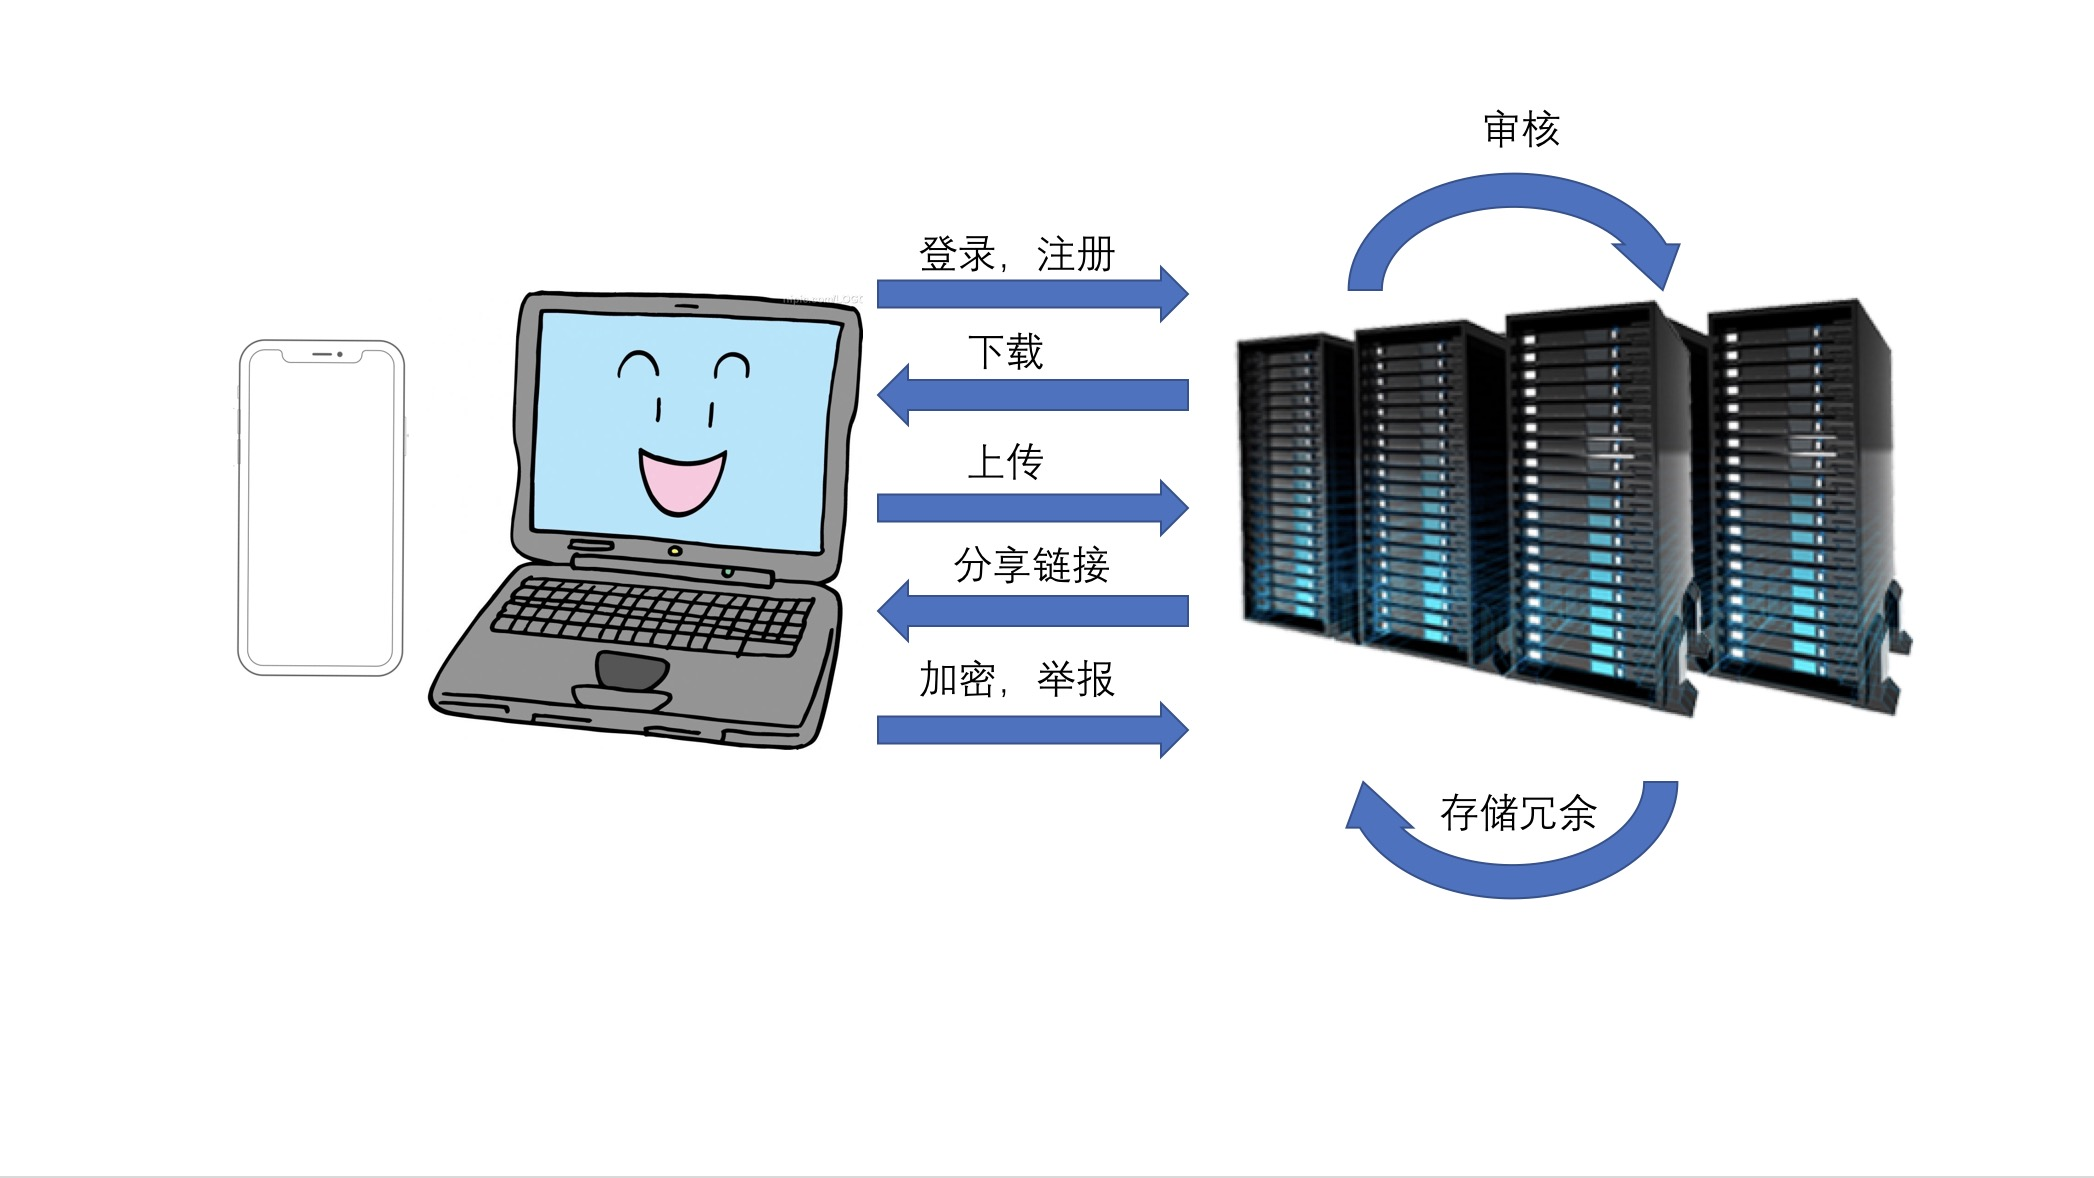
\includegraphics[width=16cm]{top.png}
\caption{顶层数据流图}\label{fig:noted-figure}
\end{figure}

\subsection{层数据流图}

在这里画出0层数据流图
 
\subsection{层数据流图}
<Draw the Level-1 DFD here>

在这里画出1层数据流图

\section{数据字典}
\subsection{数据流说明}
\subsubsection{用户信息}
来源:用户

简述:用户的基本个人信息

去向:服务器

\subsubsection{上传文件}
来源:用户

简述:用户上传到云盘中的文件

去向:服务器

\subsubsection{下载文件}
来源:服务器

简述:通过链接下载的文件

去向:用户/游客

\subsection{数据存储说明}
\subsubsection{用户信息数据表}
描述:保存每个用户相关信息的数据表

来源:用户创建,修改操作

去处:身份验证系统,指令管理系统

组成:用户名+密码

排序方式:用户名的字典序

\subsubsection{上传文件数据表}
描述:保存每个用户云盘文件的数据表

来源:用户上传的文件

去处:数据库系统

组成:用户信息+目的路径+二进制文件

排序方式:用户信息, 文件路径的字典序

\subsubsection{下载文件数据表}
描述:从云盘中下载文件的数据表

来源:数据库系统

去处:用户或游客

组成:文件链接+二进制文件

排序方式:文件名的字典序

\subsection{加工说明}
\subsubsection{验证信息合法性}
输入:用户名密码

输出:登录/注册结果

操作:对于登录请求,判断用户名是否存在。对于注册请求,判断用户名是否合法、是否已经存在、密码是否过于简单。

\subsubsection{计算密码散列值}
输入:用户名密码

输出:用户名和密码的散列值

操作:使用sha256散列值算法,通过密码(原文),用户名和随机数计算密码的散列值。

\subsubsection{权限控制}
输入:管理云端文件系统的指令

输出:返回结果(是否成功)

操作:根据用户的身份信息和文件类型,判断用户是否有权限及该指令是否合法


\end{document}
